\section{Moduł QRS\_CLASS}

\subsection{Wstęp}
Zadaniem niniejszego modułu jest klasyfikacja zespołów QRS, polegająca na wyodrębnieniu grup podobnych do siebie zespołów na podstawie przebiegu sygnału elektrokardiograficznego wraz z zaznaczonymi punktami charakterystycznymi.\newline
\begin{figure}[h]
\centering
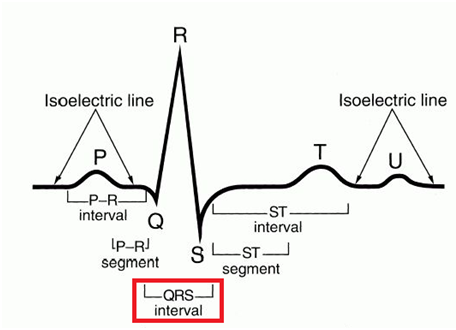
\includegraphics {QRS_CLASS/img/qrs_segment.png}
\caption{Sygnał EKG wraz z zaznaczonym zespołem QRS (kolor czerwony). Źródło: \cite{QRS_MedicalDictionary}}
\label{fig:QRS_Segment}
\end{figure}
\newline Celem klasyfikacji zespołów QRS jest określenie ośrodków bodźcotwórczych w sercu. Odmienny kształt zespołu wynika z pobudzenia o innym przebiegu, którego źródło położone jest poza podstawowym generatorem rytmu. Grupowanie zespołów odbywa się zatem ze względu na ich morfologię (kształt) przy jednoczesnym określeniu typu pobudzenia (komorowe lub nadkomorowe). Koniecznie jest także wyodrębnienie zespołów, których pobudzenia nie można określić oraz artefaktów – przebiegów omyłkowo rozpoznanych jako zespół QRS.\newpage

\subsection{Koncepcja proponowanego rozwiązania}
Klasyfikacja zespołów QRS może być wykonywana na podstawie przebiegu sygnału w analizowanym przedziale lub z wykorzystaniem wektora cech reprezentujących dany zespół. Ze względu na szybkość obliczeń w opisywanym module wykorzystano drugą metodę, opisując zespół QRS za pomocą trzech współczynników kształtu:

\begin{itemize}
\item stosunek pola powierzchni do obwodu,\newline
\begin{figure}[h]
\centering
$h_{1} = 10 \cdot\dfrac{\sum\limits_{i=0}^N \lvert s(n)\lvert}
{\sum\limits_{i=1}^N (\lvert s(n)-s(n-1)\lvert )} $
\end{figure}
\item stosunek maksymalnej prędkości do maksymalnej amplitudy,\newline
\begin{figure}[h]
\centering
$h_{2} = 10 \cdot\dfrac{\max\limits_{n=2..N} (\lvert s(n)+s(n-2)-2s(n-1) \lvert )}
{\lvert \max\limits_{n=0..N} (s(n)) - \min\limits_{n=0..N} s(n)) \lvert} $
\end{figure}
\item procentowy udział próbek, w których prędkośc przekracza 40\% prędkości maksymalnej, do długości zespołu QRS. \newline
\begin{figure}[h]
\centering
$h_{10} = \dfrac{\sum k : \{\lvert s(k)-s(k-1)\lvert > 0,4 \cdot\max\limits_{n=1..N}\lvert s(n)-s(n-1)\lvert\}}
{N} $
\end{figure}
\end{itemize}

Grupowanie poszczególnych zespołów odbywa się z wykorzystaniem algorytmu G-means, będącego ulepszeniem klasycznego algorytmu k-średnich (k-means). Główną zaletą wybranego rozwiązania jest brak konieczności określania z góry liczby klas, do których przydziela się reprezentantów.
\newline\newline Podstawowe założenie algorytmu stanowi hipoteza, że zbiór reprezentantów każdej klasy posiada rozkład Gaussa. Metoda G-średnich uruchamiana jest z niewielką początkową liczbą centroid (klas), która może być równa 1 lub więcej, w zależności od posiadanej wiedzy na temat analizowanego problemu. Następnie wykonywany jest kolejno algorytm k-średnich dopóki wszystkie klasy będą posiadały rozkład normalny lub gdy osiągnięta zostanie maksymalna liczba klas.
\newline\newline Do prawidłowego działania algorytmu konieczne jest określenie, czy dane przyporządkowane do określonej klasy mają rozkład gaussowski. Rozróżniamy zatem dwie hipotezy:
\begin{itemize}
\item dane mają rozkład normalny – klasa jest wystarczająca do reprezentacji wszystkich przedstawicieli,
\item dane nie mają rozkładu normalnego – klasa powinna być podzielona na dwie podklasy.
\end{itemize}
W celu sprawdzenia normalności rozkładu danych w określonej klasie, przeprowadzono test Andersona-Darlinga, opisany statystyką:\newline
\begin{figure}[h]
\centering
$A^2(x) = -n - \frac{1}{n}\sum\limits_{i=1}^n(2i-1)(\log(\Phi(y_{i})) + \log(1-\Phi(y_{n+1-i}))) $
\end{figure}
\begin{tabbing}
\newline gdzie: \= $n$ - liczba przedstawicieli danej klasy,\\
\> $y_{i}$ - wartości reprezentantów przekształcone do rozkładu normalnego,\\
\> $\Phi (x)$ - dystrybuanta rozkładu normalnego N(0,1).\\
\end{tabbing}

W przypadku, gdy wartości wariancji i odchylenia standardowego są szacowane, wykorzystuje się zmodyfikowaną statystykę:
\begin{figure}[h]
\centering
$A^*2(x) = A^2(x) \cdot (1+\frac{4}{n} +\frac{25}{n^2})  $
\end{figure}

Rozkład uznaje się za normalny jeżeli wartość statystyki jest mniejsza od zadanego progu tolerancji $\alpha$.\newline
Detekcja i eliminacja artefaktów następuje w dwóch etapach:
\begin{itemize}
\item wyodrębnienie próbek o zerowej długości (punkty QRS\_onset i QRS\_end pokrywają się ze sobą),
\item wykreślenie przedstawicieli klas, których odległość od danej centroidy jest większa niż dwukrotność wariancji. \newpage
\end{itemize}

\subsection{Diagramy klas}
Poniżej przedstawiono diagram głównej klasy modułu: \newline\newline
\begin{tikzpicture}
  \begin{class}[text width=10cm]{QRSClassModule}{0,0}
    \attribute{extractors : Qlist<AbstractExtractor*>}
    \attribute{clusterer : AbstractClusterer*}
    \attribute{errMsg : Qstring}
    \attribute{ecgBaselined : Qvector<double>*}
    \attribute{waves\_onset : QVector<QVector<double>::const\_iterator>*}
    \attribute{waves\_end : QVector<QVector<double>::const\_iterator>*}
    \attribute{artifactsList : Qlist<int>*}
    \attribute{runParallel : bool}
    
	\operation{setDefaultConfiguration()}
	\operation{setClusterer(clustererType : ClustererType)}
	\operation{setECGBaseline(ecg : QVector<double>*)}
	\operation{setWaves(waves\_onset : QVector<QVector<double>::const\_iterator>*, waves\_end : QVector<QVector<double>::const\_iterator>*)}
	\operation{bool setSettings(settings: QRSClassSettingd)}
	\operation{bool process()}
	\operation{QVector<QRSClass>* getClasses()}
	\operation{QString getErrorMessage()}
  \end{class}
\end{tikzpicture}\\
\newpage Klasa AbstractClusterer jest klasą bazową dla algorytmów grupowania:\newline\newline
\begin{tikzpicture}
  \begin{class}[text width=10cm]{AbstractClusterer}{0,0}
    \attribute{InitTypes{RandomPoints, KMeansPP} : enum}
    \attribute{instances : Qlist<instance>*}
    \attribute{centroids : Qlist<instance>*}
    \attribute{artifacts : Qlist<int>*}
    \attribute{initCentroids : bool}
    \attribute{maxIters : int}
    \attribute{errMsg : QString}
    \attribute{itersPerformed : int}
    \attribute{numOfClusters : int}
    
	\operation{Qlist<instance>* initializeKMeansPPCentroids(numberOfClusters : int)}
	\operation{Qlist<instance>* initializeRandomPointsCentroids(numberOfClusters : int)}
	\operation{Qlist<instance>* initializeCentroids(type : InitTypes, numberOfClusters : int)}
	\operation{virtual bool classify() = 0}
	\operation{handleArtifacts()}
	\operation{Qlist<int>* getArtifacts()}
	\operation{virtual Qlist<Instance>* getClasses() = 0}
	\operation{virtual Qlist<int>* getClassMembers(ClassNumber : int) = 0}
	\operation{virtual int getClassRepresentative(ClassNumber : int) = 0}
	\operation{virtual setInitCentroids(flag : bool)}
	\operation{virtual setInitCentroids(centroids : Qlist<Instance>*)}
	\operation{setClusteringSet(set : Qlist<Instance>*)}
	\operation{setMaxIterations(iters : int)}
	\operation{QString getErrorMessage()}
	\operation{int getPerformedIterations()}
  \end{class}
\end{tikzpicture}\\\newpage
\subsection{Rezultaty i wnioski}
\subsubsection{Działanie programu}
W zakładce "QRS Classification" wybieramy metodę klasyfikacji (G-Means lub K-Means), określając jednocześnie liczbę iteracji dla każdego algorytmu (domyślnie 1000). Algorytm wykonuje się po naciśnięciu przycisku RUN QRS\_CLASS.\newline
\begin{figure}[h]
\centering
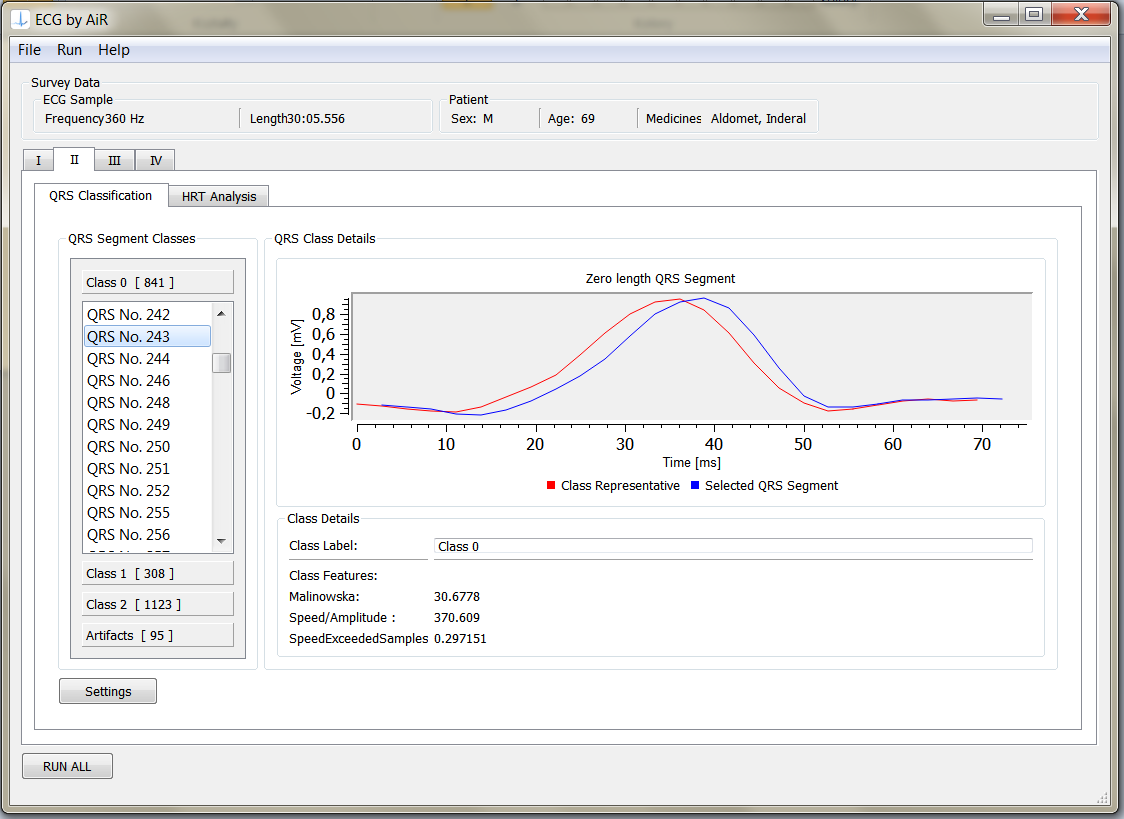
\includegraphics[width=\textwidth,keepaspectratio] {QRS_CLASS/img/screen.png}
\caption{Okno programu po wykonaniu algorytmu K-Means.}
\label{fig:QRS_Screen}
\end{figure}

\subsubsection{Możliwości rozszerzenia}
W celu  ulepszenia modułu (poprawy klasyfikacji zespołów QRS) możliwe jest dodanie kolejnego algorytmu grupującego, który dawałby możliwość porównania otrzymanych wyników. Przykładowym rozwiązaniem jest zastosowanie metody Expectation Maximization – algorytmu iteracyjnego stosowanego do tworzenia modeli danych statystycznych, możliwego do wykorzystania także gdy istnieje ryzyko niekompletnych danych.
\newline\newline Wejścia metody Expectation Maximization (EM) stanowią: wektor danych (\textit{x}), liczba klas (\textit{M}), dopuszczalny błąd (\textit{e}) oraz maksymalna liczba iteracji. Algorytm może być podzielony na dwa etapy: etap inicjalizacji i etap iteracyjny, który składa się z dwóch kroków: estymacji - expectation step (E-step) i maksymalizacji - maximization step (M-step), wykonywany iteracyjnie do czasu osiągnięcia zbieżności.
\newline\newline W kroku E-step szacuje się prawdopodobieństwo przynależności wektora do danej klasy, a następnie w kroku M-step ponownie określa się wektor parametrów rozkładu prawdopodobieństwa każdej klasy. Wykonanie algorytmu kończy się, gdy osiągnięto dopuszczalną wartość błędu lub po osiągnięciu maksymalnej liczby iteracji.

\subsubsection{Wnioski}
Klasyfikacja zespołów QRS stanowi ważny element detekcji i przetwarzania sygnału elektrokardiograficznego.  Wykonanie projektu w tej dziedzinie pozwoliło na zapoznanie się z kilkoma zaawansowanymi metodami klasyfikacji wzorców i wykorzystanie narzędzi programistycznych, które znajdują zastosowanie nie tylko w szeroko pojętej medycynie.
\newline \newline Z powodu wysokiego stopnia skomplikowania zastosowanych metod, dużej ilości czasu przeznaczonej na synchronizację modułu z pozostałymi częściami aplikacji oraz licznych problemów podczas kompilacji kodu nie udało się z powodzeniem zaimplementować dodatkowej metody klasyfikacji. Do wykonanego modułu można jednak w prosty sposób dodać nowe algorytmy, które w przyszłości posłużą do jeszcze dokładniejszej analizy zespołów QRS.